\documentclass[12pt,a4paper]{article}
\usepackage[utf8]{inputenc}
\usepackage[swedish]{babel}
\usepackage{amsmath}
\usepackage{amsfonts}
\usepackage{amssymb}
\usepackage[affil-it]{authblk}
\usepackage{subcaption}
\usepackage[innercaption]{sidecap}
\usepackage{floatrow}
\usepackage{movie15}

\RequirePackage{color,graphicx}
\usepackage{hyperref}
\definecolor{linkcolor}{rgb}{0,0.2,0.6}
\hypersetup{colorlinks,breaklinks,urlcolor=linkcolor,linkcolor = linkcolor} 
\usepackage{blindtext}
\graphicspath{{C:/Users/danne/Pictures/}}

\begin{document}

\author{Rasmus Svensson%
  \thanks{E-mail: \href{mailto:rasmus.sjobol@gmail.com}{rasmus.sjobol@gmail.com}}, \ {Daniel Holmkvist%
  \thanks{E-mail: \href{mailto:dh222kd@student.lnu.se}{dh222kd@student.lnu.se}}}}
\title{Inlämningsuppgift 1 - 1DV005}
\maketitle
\tableofcontents
\newpage
\section{Scratchuppgifter}
\subsection{Uppgift 1: Euklides algoritm}
PROBLEMLÖSNINGSSTRATEGI 
Vår implementation börjar med att fråga användaren om två tal a,b (här används  Då vill vill att $ a \geq b$ byter vi värde på dem ifall detta ej uppfylls. Sedan använder vi (pseudokod): 
WHILE b != 0         \\
 	rest = a mod b \\
	a = b \\
	b = rest \\ 
	
Först används modulus för att beräkna resten, sedan genomförs Euklides algoritm tills resten från divisionen mellan a och b är 0. Euklides algoritm säger att när resten är 0 är svaret funnet och är a, så där slutas loopen, och svaret skrivs ut. \\

%\noindent\begin{minipage}{0.3\textwidth}% adapt widths of minipages to your needs
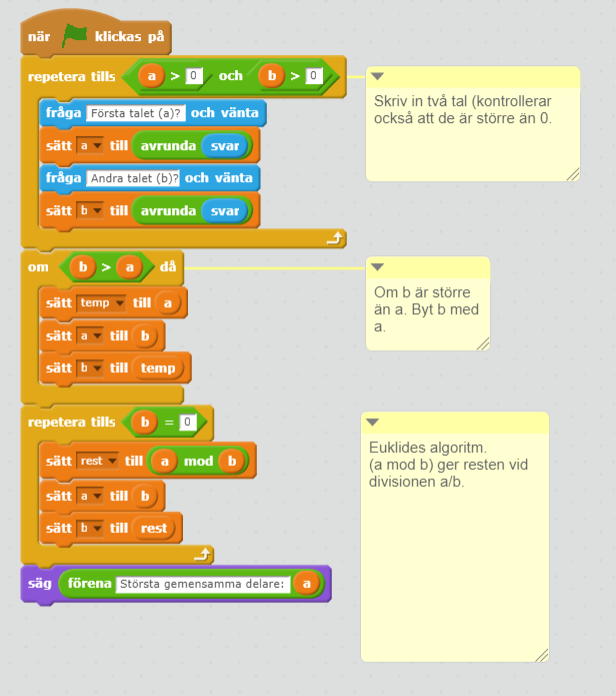
\includegraphics[scale=0.85]{euklidesimpl}

%\end{minipage}%
%\hfill%

Länk till projektet:  \\
 \url{https://scratch.mit.edu/projects/178445830/#editor }
\subsection{Uppgift 2: Binärsökning}
På denna uppgiften har vi en sorterad lista på 10 olika heltal.
Vi implementerade algoritmen rekursivt. Binärsökning jämför det mellersta elementet i en lista med det som eftersöks (här kallat nyckeln). Då finns tre fall:    \\ \\
Fall 1. Värdet på mittenelementet i listan = nyckeln. Detta medför att elementet som söks har funnits, och vi kan skriva ut dess index.  \\
Fall 2. Värdet på mittenelementet $<$ nyckeln. Eftersom listan är sorterad måste elementets som söks ha ett större indexvärde än det vi nu kollar på, således räcker det att söka igenom den halvan av listan. Mittenelementet kan också uteslutas då det redan är känt från 1) att det inte är det värdet vi söker. \\
Fall 3. Värdet på mittenelementet $>$ nyckeln. Med samma resonemang som i fall 2 kan vi söka igenom endast den halvan som har ett mindre index än mittenelementet.\\ \\
Om värdet som söks ej hittades kan samma metod kallas igen, fast med nya gränser för de index som söks. De möjliga index en nyckel kan ha halveras således varje genomkörning. Indexet på det mellersta elementet inom gränserna max,min (heltal), fås genom  $(max + min)/2$. Detta värdet kan emellertid vara ett decimaltal, således avrundas det (här: alltid neråt). 	

Om inte värdet finns med i listan kommer, vid något steg av genomsökningen värdet ligga utanför gränserna som söks, och då kan vi avbryta sökningen. 

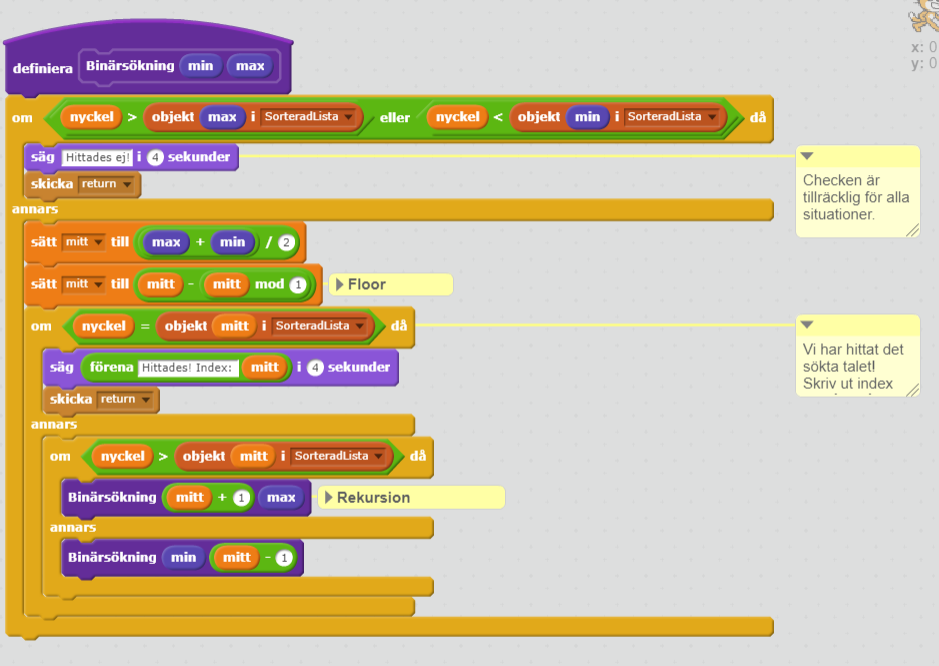
\includegraphics[scale=0.65]{binaryimpl}
\\ ``Definiera'' i Scratch liknar en metod i ett ``riktigt'' programmeringsspråk. Eftersom allt är globalt i Scratch fanns inget behov av att skicka med nyckeln eller array:n/listan.   \\
Länk till projektet: \\ \url{ https://scratch.mit.edu/projects/178458263/#editor } 
\subsection{Uppgift 3,4: Slumptal \& Urvalssortering}
För att lägga in slumpmässigt valda tal i listan används: \\ 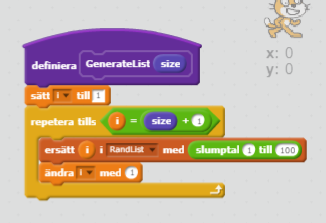
\includegraphics[scale=1]{listgen}
Vi lägger in ett tal mellan 1-100 på första platsen, sedan andra, tills vi nått slutpunkten. Detta görs här genom en 
 \\
 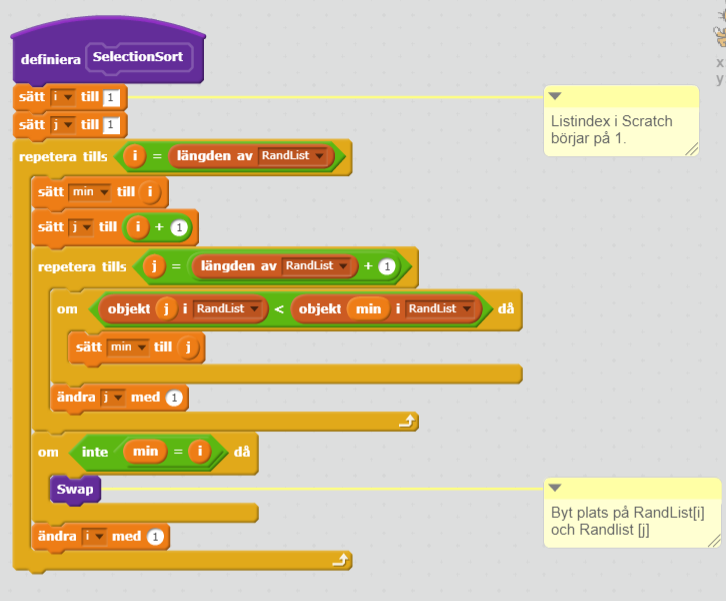
\includegraphics[scale=0.8]{selection}
\section{Tidrapport}
9/10 -2017 1h /person. 
10/10 - 2017 1h / person. 
\end{document}
